\documentclass[10pt, conference, compsocconf]{IEEEtran}
\usepackage[utf8]{inputenc}
\usepackage[brazil]{babel}
%\usepackage{hyperref}
%\hypersetup{colorlinks=false}

% *** CITATION PACKAGES ***
%
\usepackage{cite}
% *** GRAPHICS RELATED PACKAGES ***
%
\ifCLASSINFOpdf
  % \usepackage[pdftex]{graphicx}
  % declare the path(s) where your graphic files are
  % \graphicspath{{../pdf/}{../jpeg/}}
  % and their extensions so you won't have to specify these with
  % every instance of \includegraphics
  % \DeclareGraphicsExtensions{.pdf,.jpeg,.png}
\else
  % or other class option (dvipsone, dvipdf, if not using dvips). graphicx
  % will default to the driver specified in the system graphics.cfg if no
  % driver is specified.
  % \usepackage[dvips]{graphicx}
  % declare the path(s) where your graphic files are
  % \graphicspath{{../eps/}}
  % and their extensions so you won't have to specify these with
  % every instance of \includegraphics
  % \DeclareGraphicsExtensions{.eps}
\fi
% *** MATH PACKAGES ***
%
\usepackage[cmex10]{amsmath}

% *** PDF, URL AND HYPERLINK PACKAGES ***
%
\usepackage{url}

\usepackage{graphicx}

\usepackage{color}


% correct bad hyphenation here
\hyphenation{op-tical net-works semi-conduc-tor}


\begin{document}
%
% paper title
% can use linebreaks \\ within to get better formatting as desired
\title{Predição de Renda Anual}


% author names and affiliations
% use a multiple column layout for up to two different
% affiliations

\author{\IEEEauthorblockN{Leandro Luciani Tavares, Luiz Benedito Aidar Gavioli, Victor Narcizo de Oliveira Neto}
\IEEEauthorblockA{Departamento de Computação (DComp)\\
Universidade Federal de São Carlos (UFSCar) \\
18052-780, Sorocaba, São Paulo, Brasil\\
leandro.ltavares@gmail.com, luizbag@gmail.com, vnarcizo@gmail.com}
}

% make the title area
\maketitle

\begin{abstract}
Resumo, deixar para o final.

\end{abstract}

\begin{IEEEkeywords}
component; formatting; style; styling;

\end{IEEEkeywords}

\section{Introdução}
Aprendizado de máquina é atualmente um dos principais campos da computação, sendo um sub-campo da Inteligência Artificial, o qual pretende dar habilidade às máquinas de obter conhecimento e se aperfeiçoarem em determinada tarefa, sendo ela, muitas vezes, pouco trivial ou até mesmo impossível para um humano realizar devido à complexidade ou ao volume dos dados.

Nesse projeto, essa tarefa consiste em comparar o desempenho dos principais métodos de classificação estudados na disciplina de Aprendizado de Máquina: o KNN(K-vizinhos mais próximos), a Regressão Logística, as Redes Neurais Artificiais (RNA), as Máquinas de Vetores de Suporte (SVM) e o Naive-Bayes, na classificação de padrões de renda \cite{trabalho}.

A predição de padrões de renda, é uma necessidade crescente de instituições fincanceiras, como bancos, seguradoras, factories, casas de câmbio, cooperativas de crédito, entre outras. Equipadas com ferramentas e dados, as instituições tem a possibilidade de fornecer serviços personalizados para seus clientes como, por exemplo, taxas diferenciadas para clientes baseados em suas rendas anuais. Ou adequar seu modelo de negócios a determinado tipo de consumidor, sabendo-se que, por exemplo, este tem um perfil inadimplente \cite{importance}.

Em análises econômicas, prever e classificar padrões de renda é parte fundamental, dada a necessidade de estimar o desenvolvimento econômico de um país, e traçar perfis dos cidadãos, como por exemplo, qual setor da economia tem os melhores salários, qual idade tem a parcela da população que possui maior renda anual. Além de auxiliar o planejamento econômico, controle de inflação e definição de taxas de juros \cite{importance2}.

A comparação se baseia na classificação de renda dos cidadãos norte-americanos, em 2 classes: os que possuem renda inferior à 50 mil dólares anuais ou os que possuem renda superior ou igual à 50 mil dólares anuais, com base em 14 atributos. A base utilizada para comparação pode ser consultada em \cite{base} e \cite{base2}.

\section{Base de dados}
A base de dados fornecida estava, inicialmente, separada em 2 arquivos, adult\_test e adult\_data, aos quais adicionou-se uma linha de cabeçalho para importação no Matlab, unificou-se ambos arquivos para o pré-processamento. A base de dados é composta por 14 atributos e 1 atributo-alvo, que representa se a renda é inferior a 50 mil dólares anuais ou igual ou superior a 50 mil dólares anuais, sendo eles:

\begin{description}
\item[Age] \hfill \\ Atributo contínuo que representa idade;
\item[Workclass] \hfill \\ Atributo categórico que representa uma das 9 classes de trabalho;
\item[Fnlwgt] \hfill \\ Atributo contínuo;
\item[Education] \hfill \\ Atributo categórico que representa um dos 16 graus de escolaridade;
\item[Education-num] \hfill \\ Atributo contínuo relacionado ao grau de escolaridade;
\item[Marital-status] \hfill \\ Atributo categórico que representa um dos 7 estados civis;
\item[Occupation] \hfill \\ Atributo categórico que representa uma das 14 áreas de trabalho;
\item[Relationship] \hfill \\ Atributo categórico que representa um dos 6 parentescos;
\item[Race] \hfill \\ Atributo categórico que representa uma das 5 etnias;
\item[Sex] \hfill \\ Atributo categórico que representa um dos 2 gêneros possíveis;
\item[Capital-gain] \hfill \\ Atributo contínuo que representa o ganho de capital;
\item[Capital-loss] \hfill \\ Atributo contínuo que representa a perda de capital;
\item[Hours-per-week] \hfill \\ Atributo contínuo que representa as horas trabalhadas por semana;
\item[Native-country] \hfill \\ Atributo categórico que representa um das 41 nacionalidades.
\end{description}

Após o carregamento removeu-se as amostras duplicadas, resultando em um total de 48813 amostras únicas, removeu-se também amostras com atributos idênticos porém com atributo-alvo distinto, resultando em 48785 amostras.

Apresentaram-se 3615 amostras com informações ausentes para os atributos: \textbf{work-class, occupation, native-country}. Essas amostras representavam cerca de 8\% do total, portanto, optou-se por removê-las da base dados. Resultando em 45170 amostras.

Os atributos contínuos não sofreram modificações para os métodos do KNN, Regressão Logística, Redes Neurais e SVM, entretanto para o método Naive Bayes discretizou-se os valores em 10 cestas e aplicou-se a suavização de Laplace a fim de tratar cestas que não continham valores.

Os atributos categóricos foram convertidos em colunas, sendo que cada coluna representa um dos valores possíveis para o atributo original e o valor de cada uma das colunas passa a ser binário, indicando se a categoria do atributo original é a representada pela coluna.

Devido a expansão dos atributos categóricos, 3 colunas representavam atributos ausentes para 3 atributos originais. Devido à remoção das amostras com atributos ausentes, tornou-se irrelevante manter essas colunas, portanto as mesmas foram removidas. Após essas transformações os 14 atributos originais tornaram-se 105. Para o método Naive-Bayes os 14 atributos originais tornaram-se 160.

O atributo-alvo foi convertido em um atributo binário, 1 para representar a classe positiva (renda igual ou superior a 50 mil dólares anuais) e 0 para representar a classe negativa (renda inferior a 50 mil dólares anuais). \textbf{11197 amostras (24,79\%) representam a classe positiva e 33973 amostras representam a classe negativa (75,21\%).}

Implementou-se 2 tipos de normalização para todos os atributos, exceto o atributo-alvo:

\begin{description}
\item[Normalização por reescala] \hfill \\ Restringe o intervalo de valores entre 0 e 1 para um atributo, mais sensível a outliers;
\item[Normalização por padronização] \hfill \\ Garante que os valores tenham média igual a 0 e desvio-padrão igual a 1.
\end{description}

Para se permitir a visualizção dos dados, implementou-se a Análise de Componentes Principais (PCA), para redução dos 105 atributos para 3, resultando na imagem disposta na Figura \ref{fig:dados3d}, na qual a classe positiva, renda igual ou superior a 50 mil dólares anuais, é representada por \textcolor{blue}{+} e a classe negativa, renda inferior a 50 mil dólares anuais, é representada por \textcolor{red}{o}.

\begin{figure}[h]
\centering
\makebox[\columnwidth]{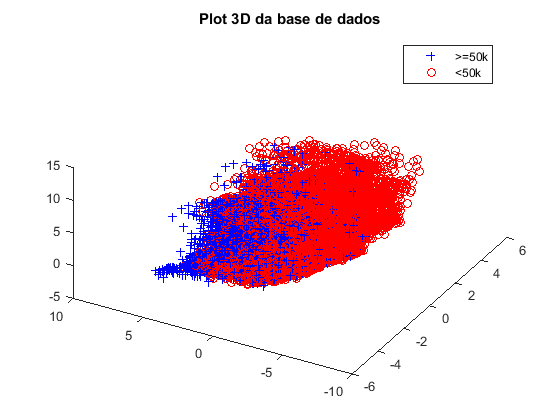
\includegraphics[width=\columnwidth]{dados3d}}
\caption{Gráfico 3D da base de dados}
\label{fig:dados3d}
\end{figure}

\section{Metodologia experimental}
\label{sec:metodologia}

Particionou-se a base de dados utilizando-se a metodologia de validação cruzada \emph{(k-fold cross-validation)}, visto que os dados não são sensíveis ao tempo. Utilizou-se 10 partições, sendo 9 delas para o treinamento e 1 para a validação, dessa forma os \textbf{conjuntos de treinamento contém 40653 amostras e os conjuntos de teste 4517 escolhidas aleatoriamente.} Uma vez selecionadas as amostras aleatórias, as partições são salvas para sempre utilizar os mesmos conjuntos de dados para treinamento e teste.

Para avaliação do poder de classificação de cada método aplicou-se as medidas mais utilizadas, como: \textbf{acurácia, F-medida, precisão e revocação, contabilizando também o tempo de treinamento e teste de cada partição.}

A fim de verificar a possibilidade de superajustamento ou subajustamento, gerou-se também os gráficos das curvas de aprendizado, realizando os treinamentos com partições incrementais, iniciando com 1 partição e finalizando com 9.

Para este relatório, utilizou-se normalização por padronização em todos os testes.

Considerou-se a possibilidade de reduzir a dimensionalidade dos dados a fim de melhorar o desemepenho do RNA e SVM.  No entanto, para manter a varância em 95\% da variância original o número de atributos não sofreu queda significativa, portanto não se aplicou a redução de dimensionalidade.

Apresentam-se aqui os parâmetros selecionados, a fim de possibilitar a reprodução dos resultados obtidos em cada método:

\subsection{KNN}

O KNN \emph{(K-vizinhos mais próximos)} é um método baseado em distâncias que consiste em selecionar os K vizinhos do conjunto de treinamento menos distantes da amostra de teste, e por distante entende-se o que apresenta a menor diferença entre os atributos.

O único parâmetro do KNN é o valor K, para o qual testou-se com os valores: 1, 3, 5, 7, 11, 21, 51. Para este relatório, selecionou-se K = 51.

\subsection{Regressão logística}

O método da regressão logística consiste em encontrar uma função \emph{(hipótese)} que classifique os atributos, minimizando o erro entre as amostras, através do ajuste dos coeficientes do polinômio \(\theta\).

Implementou-se 3 variações das hipóteses:

\begin{description}
\item[Hipótese Linear] \hfill \\ Atributos elevados a primeira potência;
\item[Hipótese Quadrática] \hfill \\ Atributos elevados a primeira e segunda potência;
\item[Hipótese Cúbica] \hfill \\ Atributos elevados a primeira, segunda e terceira potência;
\end{description}

A regressão logística ainda pode utilizar um parâmetro de regularização a fim de evitar o superajustamento ao conjunto de treinamento, balançeando a complexidade da hipótese.

Para seleção dos parâmetros testou-se, através de busca em grid, as 3 hipóteses, com parâmetro \(\lambda\) = 0, ou seja, sem regularização, e com a regularização variando de \(10^0\) a \(10^3\) com passo 1 na potência. Para este relatório, selecionou-se a hipótese linear com \(\lambda\) = 100.

\subsection{Redes Neurais Artificiais}

As Redes Neurais Artificias utilizadas foram os Perceptrons Multi-camadas que consistituem uma série de camadas massivamente conectadas de regressores logísticos, portanto, o método consiste em ajustar matrizes de coeficientes \(\theta\) a fim de minimizar o erro de classificação das amostras.

Entre os parâmetros a serem ajustados, existe a taxa de aprendizagem \(\alpha\), o número de camadas e o número de neurônios em cada camada.

Para este relatório selecionou-se \(\alpha\) = 0,06 e uma camada intermediária com 50 neurônios. Pode-se observar na literatura que somente uma camada intermediária é sufuciente para a obtenção do classificador, pois através do teorema de Cybenko a RNA tem a característica de aproximador universal.\cite{cybenko}. Dado a quantidade de atributos pela quantidade de amostras, não foi viável colocar mais uma camada intermediária, pois afetaria consideravelmente o tempo de treinamento.

Variou-se os parametros de taxa de aprendizagem de \(10^{-2}\) até \(10^{-1}\) com incremento de \(10^{-2}\). Obtendo-se o melhor desempenho e velocidade de treinamento com 0,06. A quantidade de neurônios na camada intermediária foram ajustadas com 30, 50, 100, 150, 200 e 250. Para este relatório selecinou-se 50 neurônios.

\subsection{SVM - Máquinas de vetores de suporte}

O SVM expande os atributos para um espaço de dimensão superior e encontra o hiperplano que fornece a maior margem entre os representantes de cada classe \cite{praticalSVM}. O SVM foi implementado utilizando-se a biblioteca LIBSVM \cite{libsvm}.

Os parâmetros incluem a seleção do kernel, dos coeficientes \emph{C}, que representa o parâmetro de custo (para os kernels linear, radial e polinomial) e \(\gamma\) (para os kernels radial e polinomial).

Testou-se o SVM com kernel linear, com \emph{C} com valores de \(10^{-4}\) a \(10^2\), com passo incremental 1 na potência. Para o kernel radial testou-se através de busca em grid, com \emph{C} variando de \(10^{-4}\) a \(10^2\), e \(\gamma\) variando de \(10^{-2}\) a \(10^2\) ambos com passo incremental 1 na potência.

Para este relatório selecionou-se, C = 0.01 para o kernel linear e C = 1 e \(\gamma\) = 0.01 para o kernel radial.

\subsection{Naive Bayes}

O método Naive Bayes se baseia nas probabilidades de ocorrência de cada classe, e de cada atributo individualmente sabendo a classe em que o mesmo se encontra. O método Naive Bayes se baseia apenas nas probabilidades, portanto não possuí parâmetros a serem ajustados. Aplicou-se a suavização de Laplace com o propósito de tratar possíveis cestas de valor zero.



\section{Resultados}

\subsection{KNN}

Visando obter-se as melhores acurácias e tempos de treinamento, selecionou-se o valor K = 51, obtendo-se os resultados apresentados na Tabela \ref{table:resultadosKNN}:

\begin{table}[h]
\centering
\caption{Resultados para o KNN sendo K = 51}
\vspace{0.2cm}
\begin{tabular}{c|c|c|c|c|c}
Partição & Acurácia & F-medida & Precisão & Revocação & Tempo \\
\hline
1  & 0.74607 & 0.74607 & 0.74607 & 0.74607 & 37.549 \\
2  & 0.75515 & 0.75515 & 0.75515 & 0.75515 & 37.233 \\
3  & 0.74925 & 0.74925 & 0.74925 & 0.74925 & 37.347 \\
4  & 0.75603 & 0.75603 & 0.75603 & 0.75603 & 38.548 \\
5  & 0.76179 & 0.76179 & 0.76179 & 0.76179 & 39.026 \\
6  & 0.74662 & 0.74662 & 0.74662 & 0.74662 & 38.081 \\
7  & 0.75293 & 0.75293 & 0.75293 & 0.75293 & 37.536 \\
8  & 0.75183 & 0.75183 & 0.75183 & 0.75183 & 36.817 \\
9  & 0.75803 & 0.75803 & 0.75803 & 0.75803 & 36.604 \\
10 & 0.74341 & 0.74341 & 0.74341 & 0.74341 & 36.824 \\
\hline
Média & 0.75211 & 0.75211 & 0.75211 & 0.75211 & 37.557

\end{tabular} 
\label{table:resultadosKNN}
\end{table}

\subsection{Regressão logística}

Visando obter-se as melhores acurácias e tempos de treinamento, selecionou-se a hipótese linear com um fator de regularização \(\lambda\) = 100, obtendo-se os resultados apresentados na Tabela \ref{table:resultadosRL}.

\begin{table}[h]
\centering
\caption{Resultados para a Regressão Logística sendo a hipótese linear e \(\lambda\) = 100}
\vspace{0.2cm}
\begin{tabular}{c|c|c|c|c|c}
Partição & Acurácia & F-medida & Precisão & Revocação & Tempo \\
\hline
1  & 0.86062 & 0.85909 & 0.86581 & 0.85754 & 56.846 \\      
2  & 0.86322 & 0.86180 & 0.86875 & 0.86040 & 30.724 \\      
3  & 0.85977 & 0.85811 & 0.86674 & 0.85663 & 54.428 \\      
4  & 0.86047 & 0.85899 & 0.86679 & 0.85769 & 43.907 \\      
5  & 0.86992 & 0.86865 & 0.87501 & 0.86724 & 43.519 \\      
6  & 0.86648 & 0.86497 & 0.87144 & 0.86328 & 33.003 \\      
7  & 0.86945 & 0.86790 & 0.87574 & 0.86622 & 51.874 \\    
8  & 0.86793 & 0.86640 & 0.87390 & 0.86475 & 41.304 \\      
9  & 0.86943 & 0.86804 & 0.87503 & 0.86652 & 43.230 \\      
10 & 0.86492 & 0.86317 & 0.87150 & 0.86134 & 30.503 \\
\hline
Média & 0.86522 & 0.86371 & 0.87107 & 0.86216 & 42.934

\end{tabular} 
\label{table:resultadosRL}
\end{table}

\subsection{Redes Neurais Artificiais}
	
	Visando obter-se as melhores acurácias e tempos de treinamento, selecionou-se como taxa de aprendizagem \(\lambda\) = 0,06 e quantidade de neurônios na camada intermediária com 50 elementos, obtendo-se os resultados apresentados na Tabela \ref{table:resultadosRNA}.
	
	
\begin{table}[h]
\centering
\caption{Resultados para RNA}
\vspace{0.2cm}
\begin{tabular}{c|c|c|c|c|c}
Partição & Acurácia & F-medida & Precisão & Revocação & Tempo \\
\hline
1  & 0.85583 & 0.85473 & 0.85783 & 0.85361 & 94.369 \\
2  & 0.85800 & 0.85710 & 0.85953 & 0.85617 & 102.94 \\
3  & 0.86704 & 0.86559 & 0.87189 & 0.86397 & 119.73 \\
4  & 0.86070 & 0.85964 & 0.86340 & 0.85850 & 90.938 \\
5  & 0.86618 & 0.86513 & 0.86927 & 0.86395 & 101.33 \\
6  & 0.86188 & 0.86067 & 0.86453 & 0.85935 & 105.95 \\
7  & 0.86869 & 0.86717 & 0.87472 & 0.86552 & 129.29 \\
8  & 0.86945 & 0.86829 & 0.87212 & 0.86692 & 148.67 \\
9  & 0.86756 & 0.86626 & 0.87233 & 0.86484 & 119.64 \\
10 & 0.86504 & 0.86379 & 0.86751 & 0.86239 & 113.08 \\
\hline
Média & 0.86404 & 0.86284 & 0.86731 & 0.86152 & 112.59 \\
\end{tabular} 
\label{table:resultadosRNA}
\end{table}

\subsection{Máquinas de vetores de suporte}

Visando obter-se as melhores acurácias e tempos de treinamento, selecinaram-se duas opções para o SVM, uma com kernel linear e parâmetro de custo \emph{C} = 0.01, apresentando-se os resultados na Tabela \ref{table:resultadosSVMLinear} e uma com kernel radial, parâmetros de custo \emph{C} =1 e parâmetro \(\gamma\) = 0.01, apresentando os resultados na Tabela \ref{table:resultadosSVMRadial}

\begin{table}[h]
\centering
\caption{Resultados para SVM com kernel linear e C = 0.01}
\vspace{0.2cm}
\begin{tabular}{c|c|c|c|c|c}
Partição & Acurácia & F-medida & Precisão & Revocação & Tempo \\
\hline
1  & 0.84725 & 0.84635 & 0.84835 & 0.84553 & 387.15 \\ 
2  & 0.85753 & 0.85665 & 0.85894 & 0.85575 & 371.86 \\
3  & 0.85985 & 0.85886 & 0.86134 & 0.85784 & 398.54 \\
4  & 0.85467 & 0.85379 & 0.85627 & 0.85291 & 396.04 \\
5  & 0.86017 & 0.85941 & 0.86129 & 0.85862 & 370.89 \\
6  & 0.85363 & 0.85271 & 0.85463 & 0.85186 & 371.20 \\
7  & 0.86295 & 0.86198 & 0.86457 & 0.86094 & 371.87 \\
8  & 0.86137 & 0.86044 & 0.86265 & 0.85948 & 373.39 \\
9  & 0.85854 & 0.85770 & 0.85991 & 0.85684 & 371.56 \\
10 & 0.85725 & 0.85617 & 0.85880 & 0.85508 & 371.22 \\
\hline
Média & 0.85732 & 0.85641 & 0.85867 & 0.85548 & 378.37 \\

\end{tabular} 
\label{table:resultadosSVMLinear}
\end{table}

\begin{table}[h]
\centering
\caption{Resultados para SVM com kernel radial, C = 1 e \(\gamma\) = 0.01}
\vspace{0.2cm}
\begin{tabular}{c|c|c|c|c|c}
Partição & Acurácia & F-medida & Precisão & Revocação & Tempo \\
\hline
1  & 0.84725 & 0.84635 & 0.84835 & 0.84553 & 387.15 \\ 
2  & 0.85753 & 0.85665 & 0.85894 & 0.85575 & 371.86 \\
3  & 0.85985 & 0.85886 & 0.86134 & 0.85784 & 398.54 \\
4  & 0.85467 & 0.85379 & 0.85627 & 0.85291 & 396.04 \\
5  & 0.86017 & 0.85941 & 0.86129 & 0.85862 & 370.89 \\
6  & 0.85363 & 0.85271 & 0.85463 & 0.85186 & 371.20 \\
7  & 0.86295 & 0.86198 & 0.86457 & 0.86094 & 371.87 \\
8  & 0.86137 & 0.86044 & 0.86265 & 0.85948 & 373.39 \\
9  & 0.85854 & 0.85770 & 0.85991 & 0.85684 & 371.56 \\
10 & 0.85725 & 0.85617 & 0.85880 & 0.85508 & 371.22 \\
\hline
Média & 0.85732 & 0.85641 & 0.85867 & 0.85548 & 378.37 \\

\end{tabular} 
\label{table:resultadosSVMRadial}
\end{table}

\subsection{Naive Bayes}

\begin{table}[h]
\centering
\caption{Resultados para Naive Bayes}
\vspace{0.2cm}
\begin{tabular}{c|c|c|c|c|c}
Partição & Acurácia & F-medida & Precisão & Revocação & Tempo \\
\hline
1  & 0.84255 & 0.84031 & 0.85452 & 0.83972 & 1.5254 \\
2  & 0.84731 & 0.84506 & 0.86158 & 0.84486 & 1.5465 \\
3  & 0.84693 & 0.84463 & 0.86029 & 0.84408 & 1.5446 \\
4  & 0.84498 & 0.84278 & 0.85891 & 0.84272 & 1.5119 \\
5  & 0.84862 & 0.84670 & 0.86086 & 0.84650 & 1.5206 \\
6  & 0.84920 & 0.84690 & 0.86174 & 0.84603 & 1.5198 \\
7  & 0.84499 & 0.84272 & 0.85898 & 0.84251 & 1.5126 \\
8  & 0.85428 & 0.85205 & 0.86754 & 0.85119 & 1.5395 \\
9  & 0.85367 & 0.85163 & 0.86632 & 0.85104 & 1.5342 \\
10 & 0.84597 & 0.84349 & 0.85954 & 0.84274 & 1.5229 \\
\hline
Média & 0.84785 & 0.84563 & 0.86103 & 0.84514 & 1.5278 \\

\end{tabular} 
\label{table:resultadosNB}
\end{table}

\section{Resultados gerais}

O comparativo geral entre os métodos é apresentado na Tabela \ref{table:resultadosGerais} pela média das execuções dos métodos, os melhores resultados para cada parâmetros esta destacado em negrito.

\begin{table}[h]
\centering
\caption{Resultados gerais}
\vspace{0.2cm}
\begin{tabular}{c|c|c|c|c|c}
Método & Acurácia & F-medida & Precisão & Revocação & Tempo \\
\hline
KNN                & 0.75211 & 0.75211 & 0.75211 & 0.75211 & 37.557 \\
Regresão Log. & \textbf{0.86522} & \textbf{0.86371} & \textbf{0.87107} & \textbf{0.86216} & 42.934 \\
RNA                & 0.86404 & 0.86284 & 0.86731 & 0.86152 & 112.59 \\
SVM Linear         & 0.85732 & 0.85641 & 0.85867 & 0.85548 & 378.37 \\
SVM Radial         & 0.85732 & 0.85641 & 0.85867 & 0.85548 & 378.37 \\
Naive Bayes        & 0.84785 & 0.84563 & 0.86103 & 0.84514 & \textbf{1.5278} \\
\end{tabular}
\label{table:resultadosGerais}
\end{table}




\section{Conclusão}

O trabalho apresentou uma comparação entre os principais métodos de classifição diponíveis na literatura com o objetivo de determinar se um cidadão possui renda superior ou igual a 50 mil dólares anuais ou inferior a 50 mil dólares anuais. Os atributos disponibilizado em base dados reais e publicos foram extraídos do censo norte-americano de 1994.

Desconsiderando apenas o KNN, todos os outros métodos estudados apresentaram desempenho expressivos e muito semelhantes, variando menos de 2\% entre eles, destaca-se a Regressão Logística que apresentou as melhores medidas de desempenho, atigindo uma acurácia média de 86,52\% e uma F-medida média de 86,37\%. Destaca-se também, o desempenho de tempo do método Naive Bayes, com tempo médio de treinamento igual a 1,52 segundos, cerca de 20 vezes mais rápido que o segundo colocado e praticamente 250 vezes mais rápido que o último. O KNN apresentou desempenho satisfatório, porém 10\% inferior aos métodos mais avançados, sendo o método com 

Os métodos testados apresentaram ainda resultados ligeiramente superiores aos disponíveis na literatura, o que demonstra a capacidade dos métodos empregados em resolver a tarefa de classificação de renda. Trabalhos futuros incluem um maior refinamento dos parâmetros visando desempenhos ainda superiores e a paralelização dos algoritmos a fim de realizar o treinamento em menor tempo.



% conference papers do not normally have an appendix

% use section* for acknowledgement
\section*{Agradecimentos}
Os autores gostariam de agradecer ao docente da disciplina de Aprendizado de Máquina, Prof. Dr. Tiago Agostinho Almeida pela oportunidade de colocar em prática os conhecimentos adquiridos na disciplina e pela paciência para esclarecer as dúvidas.

\nocite{*}
\bibliographystyle{IEEEtran}
\bibliography{IEEEabrv,biblio}

% that's all folks
\end{document}